\documentclass{article}
\usepackage[spanish]{babel}   
\usepackage[numbers,sort&compress]{natbib}
\usepackage{float}
\usepackage{listings}
\usepackage{graphicx} 	% Nos permite importar imagenes 
\usepackage{subfigure}
\usepackage[left=3cm,right=3cm,top=3cm,bottom=3cm]{geometry}

%-------------------------- Por si se romple la URL --------------------------
\usepackage[hyphens]{url}
\usepackage[hidelinks]{hyperref}
\hypersetup{breaklinks=true}	
\urlstyle{same}
\usepackage{cite}
%-------------------------- Por si se romple la URL --------------------------

\title{Reporte Tarea 9}
\author{Victor Alejandro Oviedo Martínez}



\begin{document}
\maketitle
\hrule

\section{Introduccón}\label{intro}
Para esta novena tarea \citep{DRA.P9} se ha estudiado el tema interacciones entre partículas, el cual tiene relación con el tema visto en la práctica 6: sistema multiagente \citep{DRA.P6}. En está practica utilizaremos el fenómeno de atracción y repulsión entre partículas eléctricamente cargadas, tendremos $n$ partículas con cargas eléctricas  entre [-1, 1] distribuida independiente mente y normal mente al azar. Por lo tanto, partículas con cargas del mismo signo tendrán una fuerza de repulsion mientras partículas de signos opuestos se atraerán, en cuanto a la magnitud de la fuerza, será proporcional a la magnitud de las cargas y inversamente proporcional a la distancia euclideana entre las partículas. La posición de las partículas esta representada por sus coordenadas en $(x, y)$, y cada valor es asignado con distribución normal con un rango [0, 1]. Una vez teniendo las condiciones iniciales, tendremos un cuadro unitario bidimensional con $n$ partículas cargadas eléctricamente, con distribución normal, por lo tanto, para realiza su simulación es necesario tener en cuenta que cada partícula es afectada por todas las demás partículas restantes, así como esta afecta a todas las demás. Por lo tanto, se tendrá que evaluar los efectos de las fuerzas individuales de todas las partículas sobre un partícula en específico, esto para obtener una fuerza resultante y poder repartir esta fuerza por medio del factor de descuento $\delta$ en sus componentes de desplazamiento $\Delta{x}$ y $\Delta{y}$. Una vez hecho este procedimiento podremos agregar el desplazamiento $\Delta{x}$ y $\Delta{y}$ a la posición $x, y$ de cada partícula. Repitiendo este procedimiento podremos visualizar el movimiento de las partículas ocasionado por las cargas eléctricas.\\






 

\section{Desarrollo}

Para esta novena tarea se ha planteado el siguiente problema: Agrega a cada partícula una masa y haz que la masa cause fuerzas gravitacionales (atracciones) además de las fuerzas causadas por las cargas. Estudia la distribución de velocidades de las partículas y verifica gráficamente que esté presente una relación entre los tres factores: la velocidad, la magnitud de la carga, y la masa de las partículas. Toma en cuenta que la velocidad también es afectada por las posiciones.

Para el desarrollo de esta tarea se a utilizado el código ejemplo proporcionado por \citet{DRA.Code}, el cual tiene el propósito de mostrar la simulación con las características ya mencionadas en la introducción. 
Este código será tomando como base para ser modificado y entregar las características de esta tarea.\\

La antes de empezar con la edición del código empezó observando que el código \citep{DRA.Code} presenta comportamientos fuera de lo normal, esto a causa de la actualización de la librería multiprocessing, por lo tanto, se tomo la decisión de eliminar el uso de multiprocessing.\\

Empezando con la edición, se ha agregado la variable \texttt{m} a la parte en la que se generan los valores para el dataframe, así como variables derivadas de \texttt{m} para su acondicionamiento.



\begin{lstlisting}[language=Python]
n = 50
x = np.random.normal(size = n)
y = np.random.normal(size = n)
c = np.random.normal(size = n)
m = np.random.normal(size = n)
xmax = max(x)
xmin = min(x)
x = (x - xmin) / (xmax - xmin) # de 0 a 1
ymax = max(y)
ymin = min(y)
y = (y - ymin) / (ymax - ymin)
cmax = max(c)
cmin = min(c)
c = 2 * (c - cmin) / (cmax - cmin) - 1 # entre -1 y 1
g = np.round(5 * c).astype(int)
mmax = max(m)
mmin = min(m)
m = (10 * (m - mmin) / (mmax - mmin) - 1)  # entre 0 y 10
m = np.round(m).astype(int)
m = abs(m * 10)
p = pd.DataFrame({'x': x, 'y': y, 'c': c, 'g': g, 'm': m})
 \end{lstlisting}
 
 Luego se ha agregado la función  \texttt{fuerzaG(i)}, esta con el fin de obtener la fuerza de gravedad generada por la variable \texttt{m} de las partículas a evaluar. Esta fuerza $F_g$ esta dada por la ecuación \ref{eq:e1} (ley de gravitación universal). Donde: $G= 6.674\times10^{-11}$ (constante de gravitación universal).
 
 \begin{equation}
 \label{eq:e1}
F_g= G\frac{m_1 m_2}{r^{2}} 
\end{equation}

En la función \texttt{fuerzaG(i)} a las variables \texttt{fgx} y \texttt{fgy} son multiplicadas para tener fuerzas mayores, ya que al no realizar la multiplicación los valores son muy pequeños para apreciar las fuerzas de las masas.\\
 
 \begin{lstlisting}[language=Python]
def fuerzaG(i):
    pi = p.iloc[i]
    xi = pi.x
    yi = pi.y
    mi = pi.m
    fgx, fgy = 0, 0
    for j in range(n):
        pj = p.iloc[j]
        xj = pj.x
        yj = pj.y
        mj = pj.m
        dx = xi - pj.x
        dy = yi - pj.y
        factor = (G * ((mi * mj) / (sqrt((dx**2) + (dy**2)) + eps)**2))
        fgx = dx * factor
        fgy = dy * factor
    return(fgx*1000000, fgy*1000000)
 \end{lstlisting}
 
 
 También ha creado la función \texttt{suma(f, fg)}, esta con el fin de sumar las fuerzas generadas por las cargas eléctricas y las fuerzas generadas por las masas, devolviendo el resultado en el mismo formato que ya se tenia.
 
 \begin{lstlisting}[language=Python]
def suma(f, fg):
    sumax = []
    sumay = []
    for v in range(n):
        FX= f[v][0]
        FGX= fg[v][0]
        sumax.append(FX + FGX)

        FY = f[v][1]
        FGY = fg[v][1]
        sumay.append(FY + FGY)

    return list(zip(sumax,sumay))
 \end{lstlisting}
 
 Cómo se mencionó con anterioridad se a eliminado el multiprocesamiento, y por lo tanto se ha  reestructurado el código.
 
  \begin{lstlisting}[language=Python]
if __name__ == "__main__":

    for t in range(tmax):

        f = []
        fg = []
        Actx = []
        Acty = []
        q = 0
        Q = 0
        for i in range(n):
            f.append(fuerza(i))
            fg.append(fuerzaG(i))

        F = suma(f, fg)

        delta = 0.02 / max([max(fabs(fx), fabs(fy)) for (fx, fy) in F])

        for v in F:
            Actx.append(actualiza(p.x[q],v[0],delta))
            q = q + 1
        p['x'] = Actx

        for v in F:
            Acty.append(actualiza(p.y[Q],v[1],delta))
            Q = Q + 1
        p['y'] = Acty


        fig, ax = plt.subplots(figsize=(7.5, 6.5), ncols=1)
        pos = plt.scatter(p.x, p.y, c = p.g, s = m, cmap = palette)
        handles, labels = pos.legend_elements(prop="sizes", alpha=0.5)
        legend2 = ax.legend(handles, labels, loc="upper right", title="Masa")
        fig.colorbar(pos, ax=ax)
        plt.xlabel('X')
        plt.ylabel('Y')
        plt.xlim(-0.1, 1.1)
        plt.ylim(-0.1, 1.1)
        plt.title('Paso {:d}'.format(t + 1))
        fig.savefig('p9p_t' + format(t + 1, '0{:d}'.format(digitos)) + '.png')
        plt.close()
 \end{lstlisting}

Hasta esta parte, el código tiene la capacidad de realiza la simulación 
con masas, sin embargo dadas las características de la tarea, es
necesario comparar las diferencias entre la simulación con y sin masa,
por lo tanto se pretende agregar al código una copia del dataframe 
\texttt{p} para poder realizar dos simulaciones diferentes con las mismas 
condiciones iniciales, de esta forma se podrá notar diferencia entre 
sistemas. Del mismo modo se agregara código para realizar el calculo de 
velocidades.\\

Para realizar dos simulaciones (con y sin masa) a sido necesario duplicar 
las condiciones iniciales y por lo tanto dos dataframes, tener dos 
funciones \texttt{fuerza(i)} y  \texttt{fuerza2(i)}, esto ya que cada función 
obtiene sus valores de diferente dataframe. En cuanto al proceso de 
repetición de cada simulación, tenemos que en este caso se simulará 
primero el sistema con masa y después el sistema sin masa, para por 
último generar las graficas de la variación de la velocidad. Por lo tanto, 
tendremos que agregar código para el cálculo de la velocidad, para esto 
se ha agregado fa función \texttt{velocidad(x0, y0, x1, y1)}, y ademas se a 
agregado los dataframe \texttt{Antiguop} y \texttt{Antiguop2}, estos 
últimos dos con la finalidad de tener una memoria de las posiciones 
antiguas y poder realizar él calculo de velocidad.\\

  \begin{lstlisting}[language=Python]
  
def velocidad(x0, y0, x1, y1):
    return (sqrt(((x1 - x0)**2) + ((y1 - y0)**2) + eps))
    
 \end{lstlisting}

Habiendo hecho lo ya mencionado tendremos un programa el cual puede simular los dos sistemas,  por lo tanto podremos comparar los cambios generados de los dos sistema. Este código tiene 2 variantes, en la primer variante el código podrá entregar imágenes para la visualización de la simulación, mientras tanto, la segunda variante entrega una gráfica para la visualización del comportamiento de la velocidad en cada tiempo de la simulación y una dispersión de los componentes de los dataframes. 

Para el desarrollo de esta tarea se utilizó la pagina \citep{DRA.Code}.


\section{Conclusión}

Cómo resultado, tenemos la figura \ref{f1} en la cual se puede observar el comportamiento de las dos simulaciones con las mismas características iniciales, por lo tanto, podemos observar las diferencias que causa la variable de la masa en la simulación. Para observar la simulación completa se tienen los archivos \texttt{Con-masa.gif} y \texttt{Sin-masa.gif}.

\begin{figure}[H]
\centering
\subfigure[Simulación sin masa, tiempo: 0.]{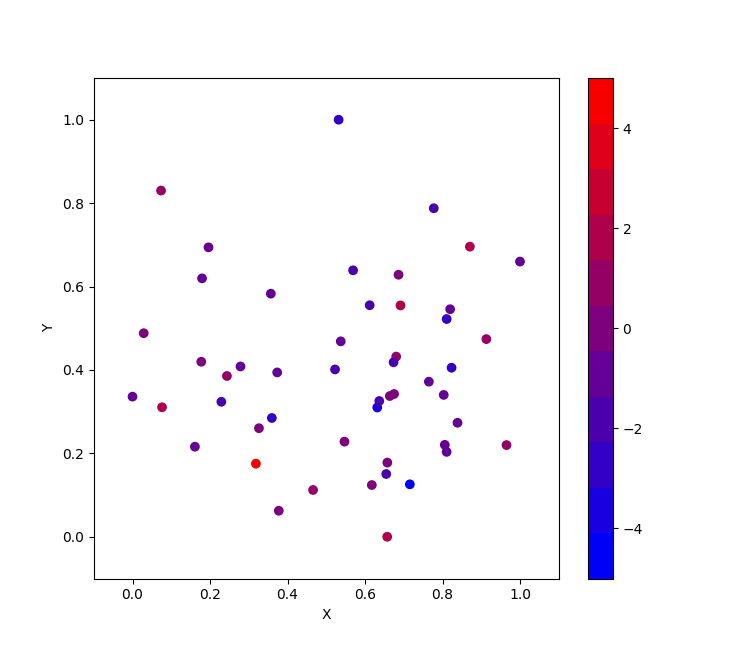
\includegraphics[width=75mm]{/Users/victor/Desktop/p9p_2t0.png}}
\subfigure[Simulación con masa, tiempo: 0.]{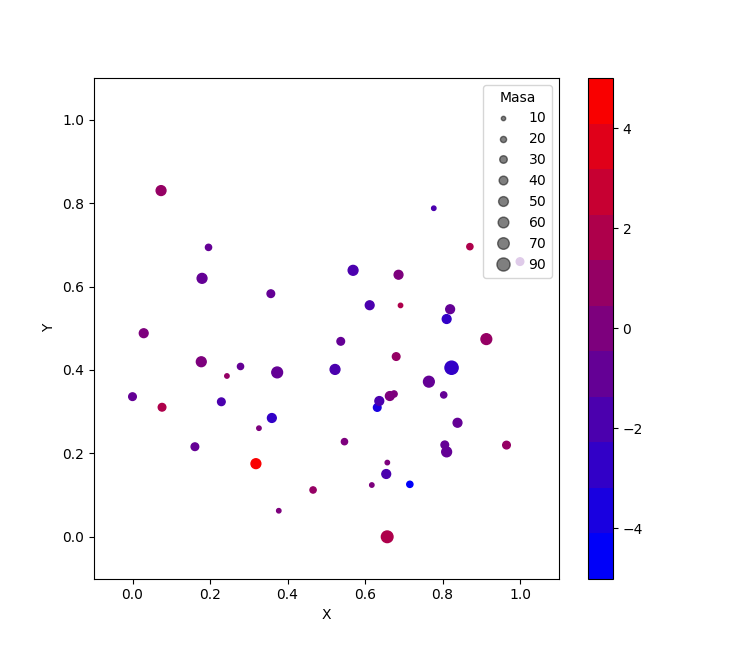
\includegraphics[width=75mm]{/Users/victor/Desktop/p9p_t0.png}}
\subfigure[Simulación sin masa, tiempo: 75.]{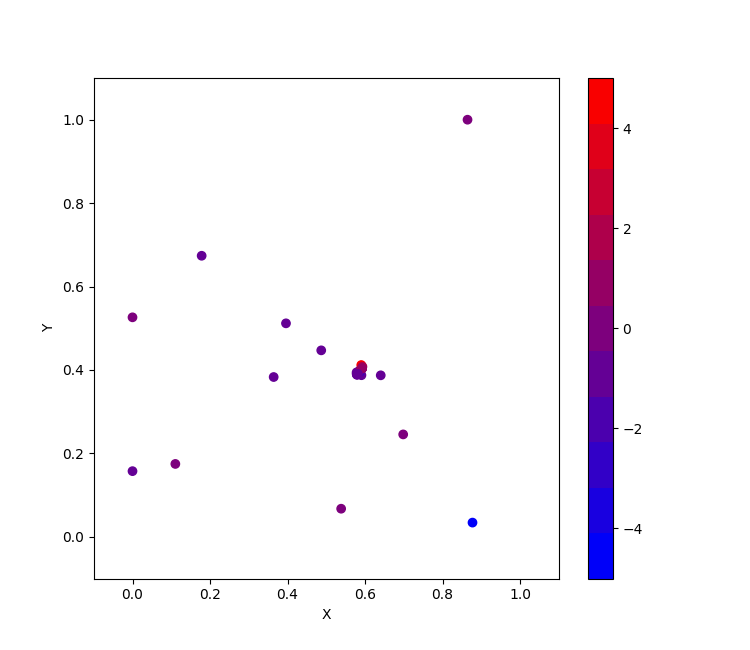
\includegraphics[width=75mm]{/Users/victor/Desktop/p9p_2t075.png}}
\subfigure[Simulación con masa, tiempo: 75.]{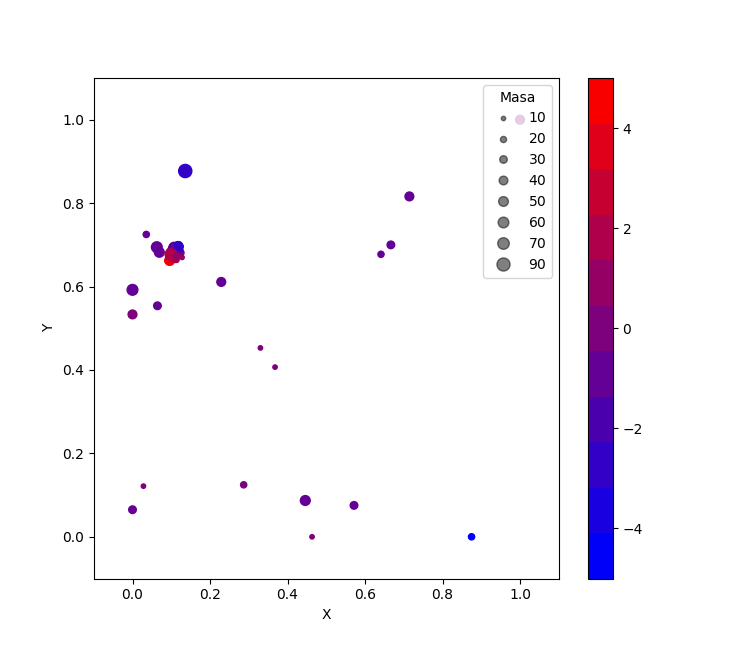
\includegraphics[width=75mm]{/Users/victor/Desktop/p9p_t075.png}}
\caption{Comparaci\'on entre simulaci\'on con y sin masa.} 
\label{f1}
\end{figure}

En cuanto a la medición de la diferencias de velocidad entre las dos simulaciones se tiene la figura \ref{f2}, en está se puede observar diferentes simulaciones de las cuales podemos concluir que las simulaciones sin la masa tienen comportamientos con velocidades mayores, mientras que las simulaciones con masa tienen menor velocidades. Esto se puede complementar con los gifs \texttt{Con-masa.gif} y \texttt{Sin-masa.gif}, en donde la simulación con masa podemos ver movimientos mas lentos en comparación a la simulación sin masa en donde una vez se juntan la mayoría de las partículas la velocidad parecería que aumenta.

\begin{figure}[H]
\centering
\subfigure[Ejemplo 1.]{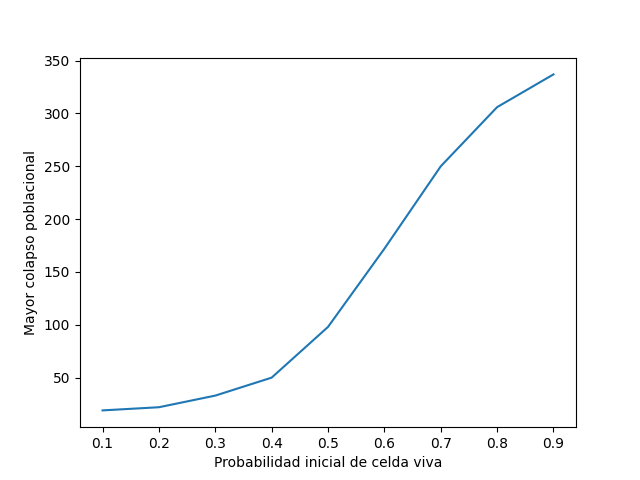
\includegraphics[width=75mm]{/Users/victor/Desktop/Figure_1.png}}
\subfigure[Ejemplo 2.]{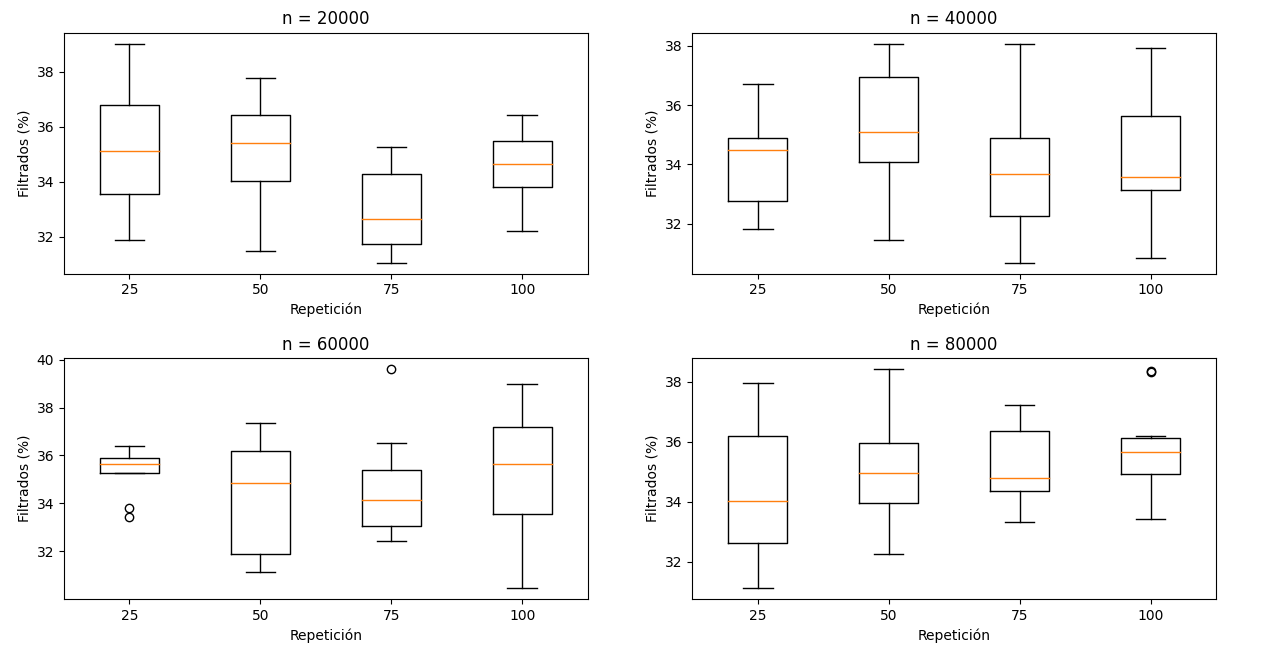
\includegraphics[width=75mm]{/Users/victor/Desktop/Figure_2.png}}
\subfigure[Ejemplo 3.]{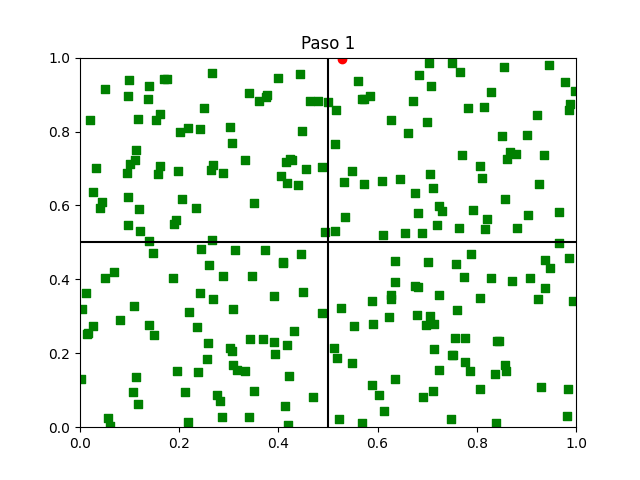
\includegraphics[width=75mm]{/Users/victor/Desktop/Figure_3.png}}
\subfigure[Ejemplo 4.]{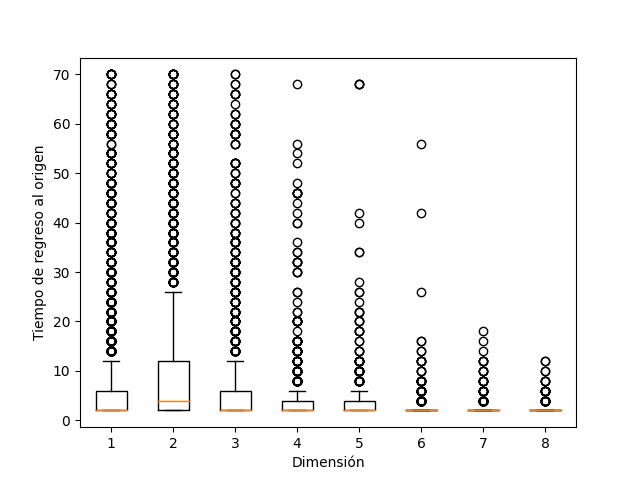
\includegraphics[width=75mm]{/Users/victor/Desktop/Figure_4.png}}
\caption{Ejemplos (Velocidad promedio VS Tiempo).} 
\label{f2}
\end{figure}

Por último, tenemos la figura \ref{f3} en la cual se observan la dispersión de las variables para las dos simulaciones, y dos tiempos diferentes (inicial y final), para el tiempo final se ha agregado la variable velocidad, de esta forma podremos observar la dispersión de las variables al inicio y al final de las simulaciones.

\begin{figure}[H]
\centering
\subfigure[Simulación sin masa, tiempo: 0.]{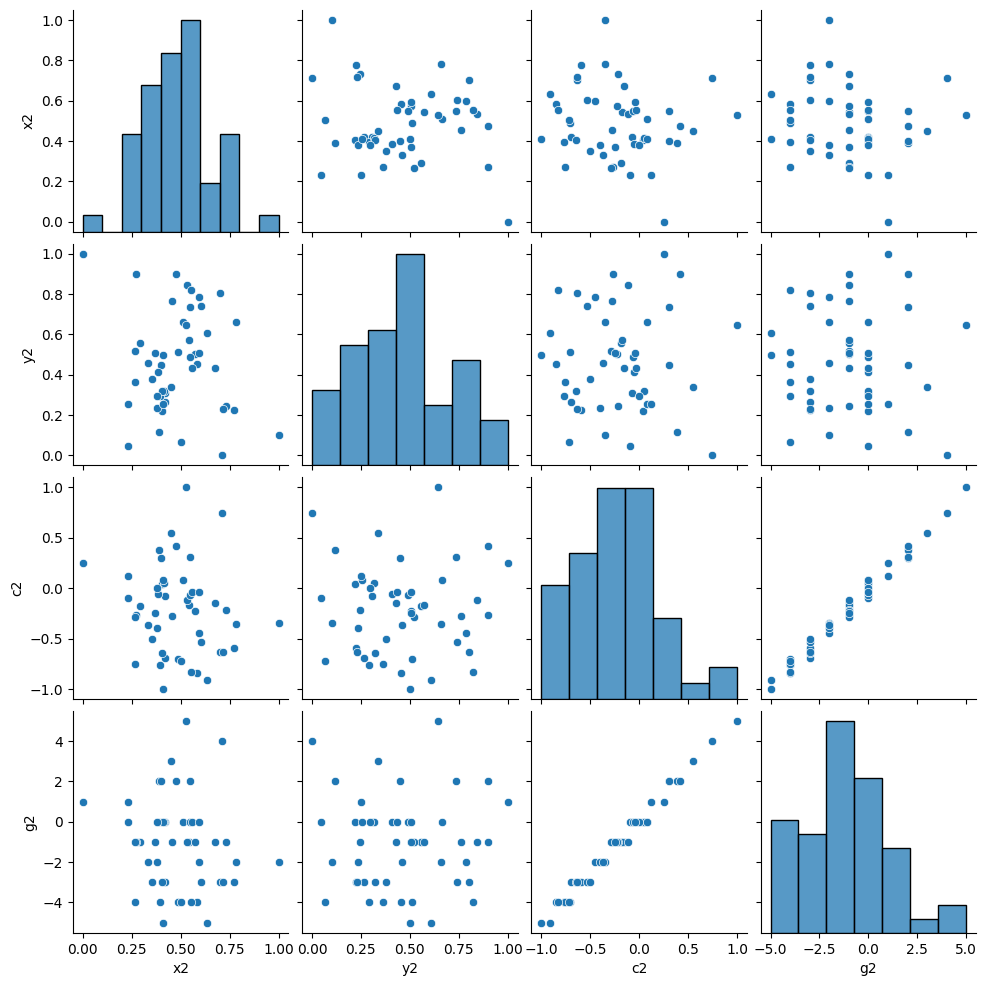
\includegraphics[width=75mm]{/Users/victor/Desktop/outputinicial2.png}}
\subfigure[Simulación con masa, tiempo: 0.]{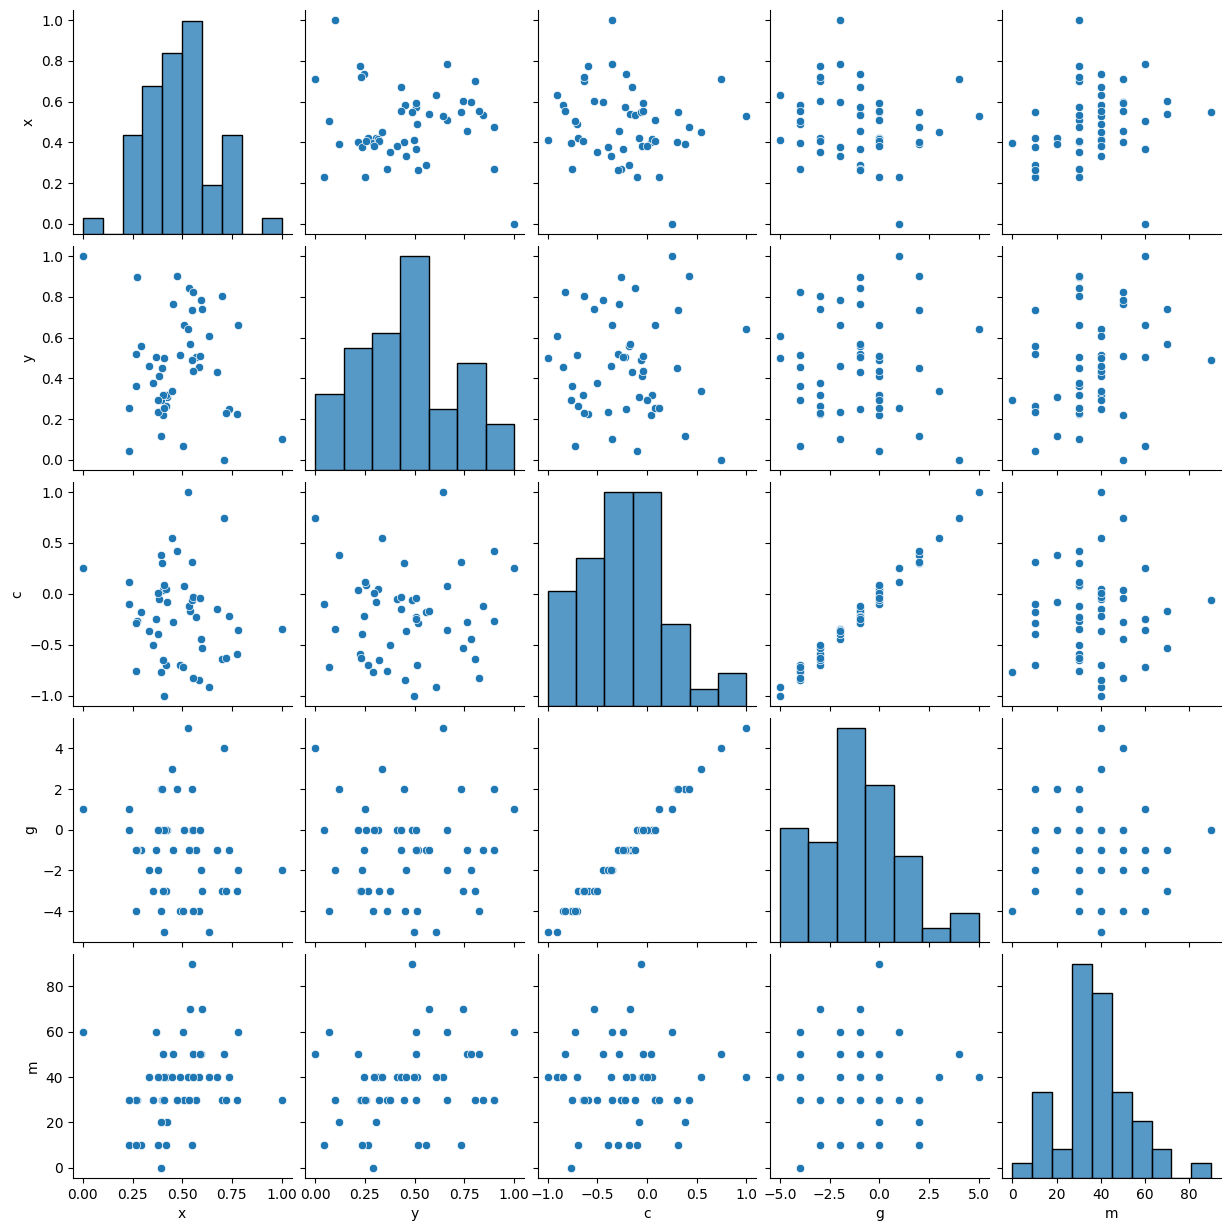
\includegraphics[width=75mm]{/Users/victor/Desktop/outputinicial.png}}
\subfigure[Simulación sin masa, tiempo: 75.]{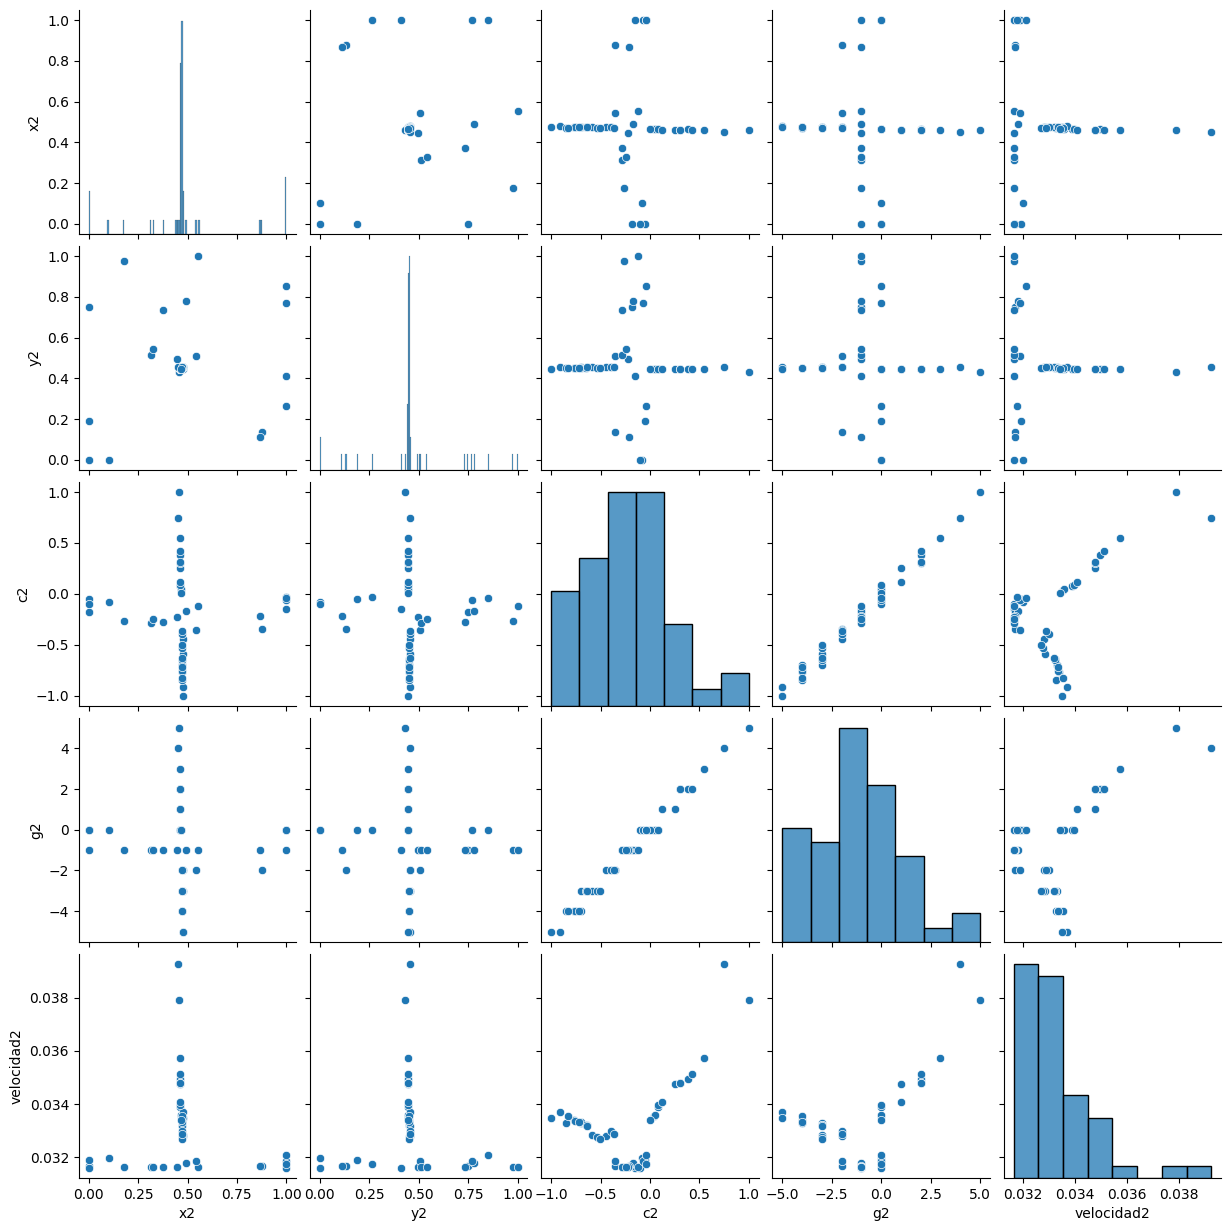
\includegraphics[width=75mm]{/Users/victor/Desktop/output2.png}}
\subfigure[Simulación con masa, tiempo: 75.]{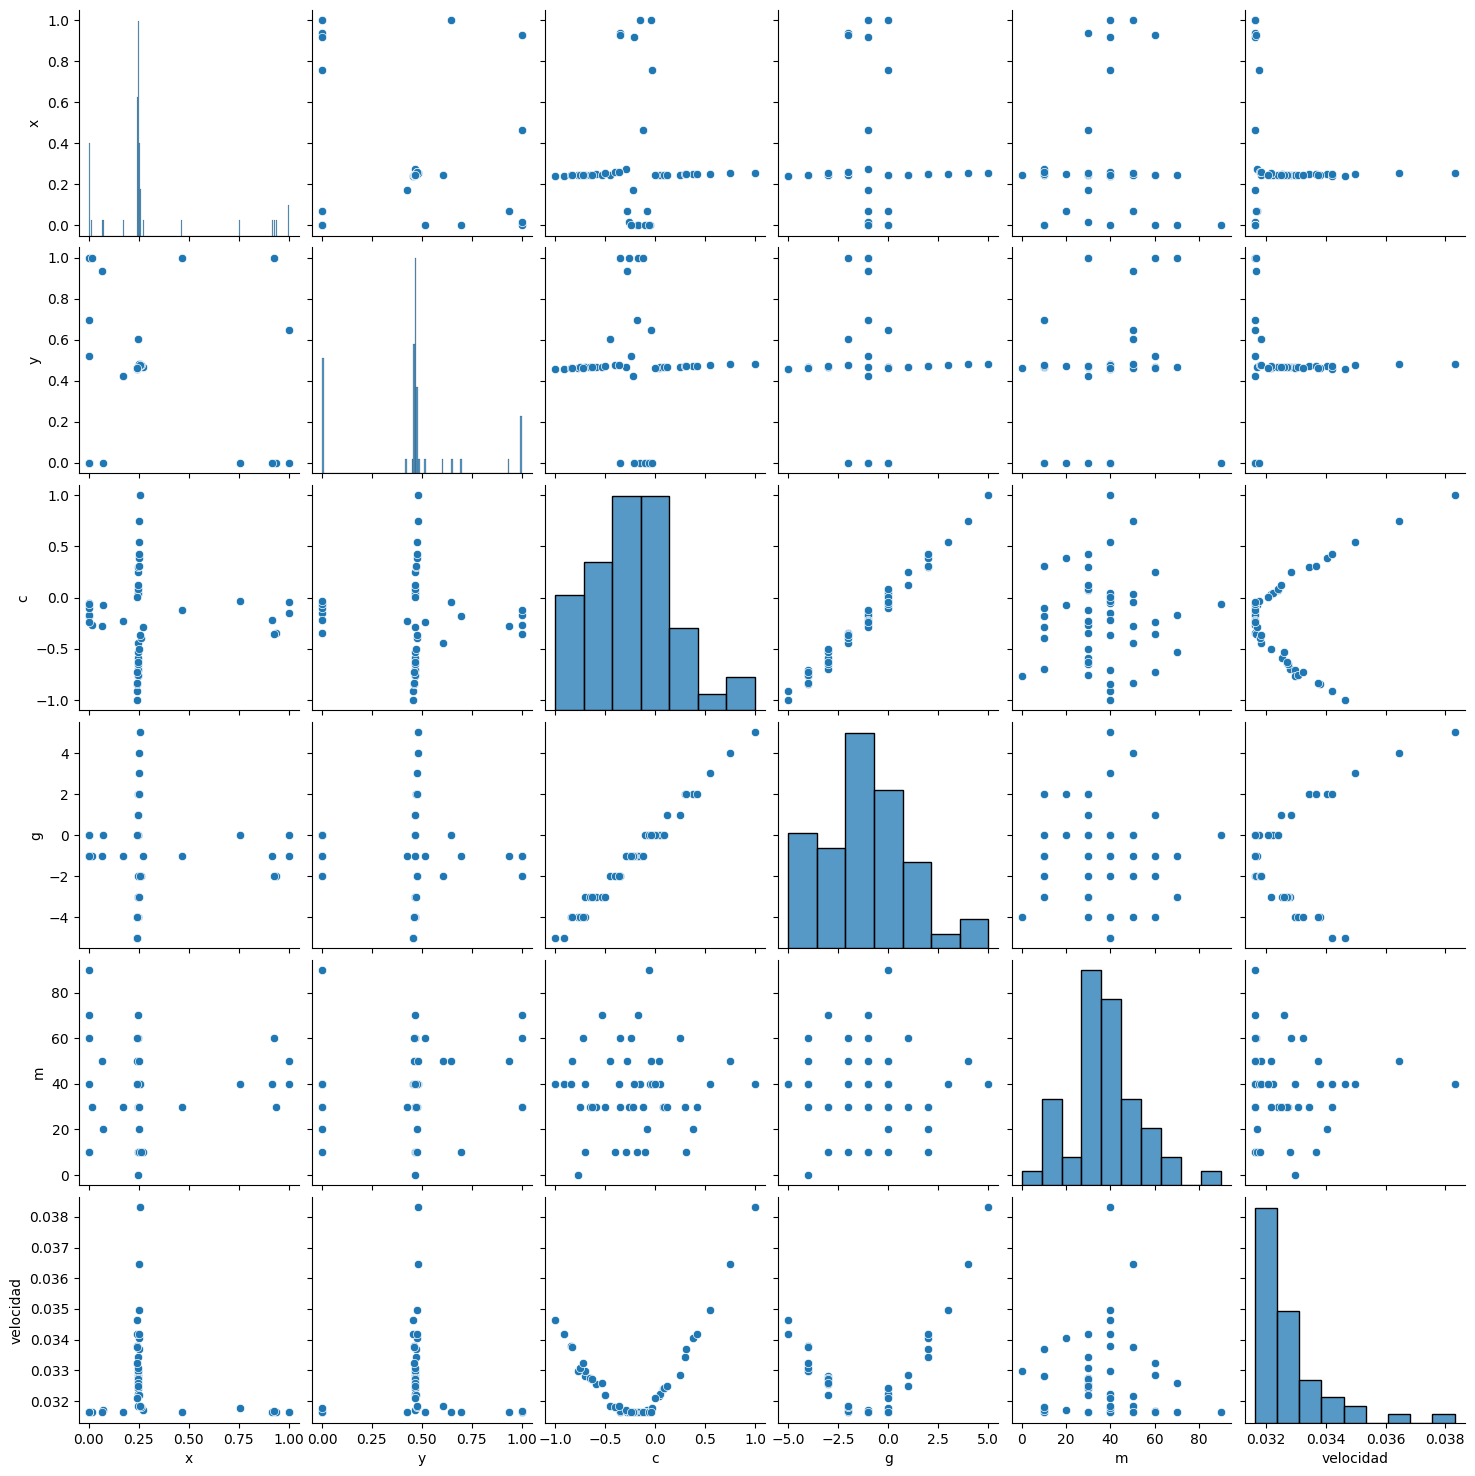
\includegraphics[width=75mm]{/Users/victor/Desktop/output.png}}
\caption{Comparaci\'on entre simulaci\'on con y sin masa.} 
\label{f3}
\end{figure}


Cómo conclusión, se ha podido comprobar el efecto que causa la masa en el comportamiento de la velocidad y por ende la posición de las partículas. Es importante tomar en cuenta todas las condiciones iniciales ya que en base a ellas la simulación se comportará de diferente manera, sin embargo, se detecto que cuando la masa esta presente en las simulaciones la velocidad de las partículas tiende a ser menor.\\

%-------------------------- Por si se rompe la URL --------------------------
\Urlmuskip=0mu plus 1mu\relax
%-------------------------- Por si se rompe la URL --------------------------
\bibliography{ref.Tarea9.bib}
\bibliographystyle{plainnat}

\end{document}